% =========================================================================
%  main_v3.tex — the RECONSTRUCTED paper 1 (JFM-2026-1781 resubmission)
%  Sharma & Kerstein.  Fresh skeleton, transplanted organs:
%  V2 (Main_submission_V2.tex) is FROZEN as the quarry — transplant sources
%  are named per section as  %% TRANSPLANT: <source> — <what/how much>.
%  Structure follows docs/REVISION_MAP_jfm1781.md section 5 (spine = the
%  single-line closure).  The LE-consequence section is DETACHABLE
%  (Option C -> S) and is written LAST.
%  Build: latexmk -pdf main_v3.tex
% =========================================================================
\documentclass[lineno]{JFM-FLM_Au}

\usepackage{xcolor}
\usepackage{tikz}
\usetikzlibrary{calc,arrows.meta}
\usepackage{subcaption}

\definecolor{jfmblue}{RGB}{0,56,168}
\def\xshift{1.5}

\hypersetup{
  colorlinks=true,
  citecolor=blue,
  linkcolor=jfmblue,
  urlcolor=jfmblue
}

\newtheorem{lemma}{Lemma}
\newtheorem{corollary}{Corollary}
\newtheorem{proposition}{Proposition}

\newenvironment{proof}
  {\par\noindent\textit{Proof.}\ }
  {\hfill$\Box$\par}

\newcounter{assumption}
\renewcommand{\theassumption}{A\arabic{assumption}}

\newenvironment{assumption}[1]{%
  \refstepcounter{assumption}%
  \par\medskip
  \noindent\textbf{Assumption~\theassumption\ (#1).}\ %
}{%
  \par\medskip
}

\lefttitle{Sharma and Kerstein}
\righttitle{Journal of Fluid Mechanics}

%% TODO(title): working title; alternatives in docs/REVISION_MAP section 5.
\title{Strain-coupled one-dimensional turbulence: a single-line closure for
the rapid pressure--strain and its measured limits}

\author{Sparsh Sharma\aff{1} \and Alan R. Kerstein\aff{2}}

\affiliation{\aff{1}German Aerospace Center (DLR), 38108 Braunschweig, Germany
\aff{2}Consultant, Danville, CA 94526, USA}

\corresau{Sparsh Sharma, sparsh.sharma@dlr.de}

\begin{document}
\maketitle

\begin{abstract}
%% PROVISIONAL — rewrite last (map task M4).  Must claim ONLY:
%%  (1) strain-coupled ODT formulation, invariants preserved (V2 claims OK);
%%  (2) the single-line closure: exact obstruction stated, sharp LOS bounds,
%%      A1 measured (exact for axisymmetric distortion, quantified error
%%      under plane strain) — NOT "a closed functional";
%%  (3) the correct linear reference: exact projected RDT is broadband, NOT
%%      rigid translation (Referee 3.1 was right; own calculation);
%%  (4) independent spectral benchmark: strained-box DNS + exact-RDT
%%      companions, three-way comparison; kappa-uniformity deficiency
%%      measured, distance-from-linear-theory envelope vs Sk/eps;
%%  (5) scale-local relaxation (hierarchical kernels) as the measured
%%      constructive direction.  NO claim that the deficiency is fixed.
The rapid distortion of turbulence by a mean strain is central to flows
from wind-tunnel contractions to the stagnation regions of lifting
surfaces, yet its economical prediction founders on a closure problem: the
rapid pressure--strain term is a nonlocal three-dimensional spectral
integral, while affordable models evolve at most one-dimensional or
single-point information. We present a strain-coupled formulation of
one-dimensional turbulence (ODT) and, as its analytical core, a systematic
treatment of what a single line of turbulence data determines about the
rapid pressure--strain term: the obstruction to a single-line closure is
stated exactly, sharp bounds on the rapid term are derived from line data
alone, and the closure assumption of axisymmetry about the line is not
assumed but measured---it is exact for axisymmetric distortion and its
plane-strain error is quantified as a function of accumulated strain.
A strained-box direct numerical simulation with an exact rapid-distortion
companion provides the independent spectral benchmark: it shows that the
correct linear reference for line-projected spectra is broadband rather
than a rigid spectral translation, and a three-way comparison localises
the model's remaining deficiency in its wavenumber-uniform rapid
kinematics, quantified by a distance-from-linear-theory envelope as a
function of strain rapidity. Hierarchical application of the model's
energy-redistributing kernel to eddy sub-scales is shown to supply the
measured missing ingredient---scale-local relaxation---where it reaches
the scales of the imbalance.
\end{abstract}

\begin{keywords}
%% chosen at submission
\end{keywords}

% =========================================================================
\section{Introduction}\label{sec:intro}
% =========================================================================
%% TRANSPLANT: V2 sec:intro — ~30%: the LE-noise motivation paragraph and
%%   the ODT lineage paragraph survive in compressed form.
%% REWRITE: novelty statement (R1 minor: do not overstate distortion-
%%   before-LE novelty; cite dos Santos et al., Ribeiro et al., Piccolo
%%   et al.).  Adopt Sagaut & Cambon 2018 ch.8 as the RDT reference spine
%%   (R2); prune sound-radiation and shock-turbulence citations (R2).
%% NEW: one paragraph stating the paper's arc: formulation -> correct
%%   linear reference -> independent benchmark -> what a line determines
%%   (bounds, measured A1) -> measured limits -> scale-local relaxation.
%% BIB: add SagautCambon2018, dosSantos, Ribeiro, Piccolo keys to jfm.bib.

\emph{[M4: introduction rewrite — see markers above.]}

% =========================================================================
\section{Strain-coupled one-dimensional turbulence}\label{sec:formulation}
% =========================================================================
%% TRANSPLANT: V2 sec:formulation (strain forcing + admissibility,
%%   sec:rapid-kernel operator, sec:domain-strain, sec:summary) — ~80%,
%%   trimmed.  R1 praised this part; keep the derivations.
%% FOLD IN: the essentials of V2 sec:odt (background) compressed to ONE
%%   review subsection with citations (R2: "a clear review of the JFM 2001
%%   paper would be better" — do exactly that); drop V2 sec:odt-standard's
%%   five subsubsections.
%% DEMOTE: Propositions 1-2 presented as consistency checks (R1 minor).

\emph{[M-formulation: transplant per markers.]}

% =========================================================================
\section{Verification against rapid-distortion theory}\label{sec:verification}
% =========================================================================
%% TRANSPLANT: V2 sec:verification (canonical strains, sec:onset,
%%   sec:finite-strain, upwash necessity, sec:level1a) — ~60%, figures
%%   consolidated; the onset check and Level-1a verification carry the
%%   "implementation is exact" burden in fewer pages.
%% ALSO: Lee & Reynolds moment-level comparison lands HERE, compressed
%%   (V2 sec:lr-validation minus its long S*-parameter discussion; the
%%   b11 finite-Re discussion survives as one paragraph).  R2 asked why
%%   L&R 1985 at all: answer in one sentence (resolvable Re on a line;
%%   graded reference curves) and lean on the in-house DNS for spectra.

\emph{[M-verification: transplant per markers.]}

% =========================================================================
\section{The linear reference and the distorted spectrum}\label{sec:val-spectrum}
% =========================================================================
%% ASSEMBLED from M2 material (final-form, transplanted below) + V2
%%   sec:spec-bvc (reframed version) + a compressed CMK comparison.
%% ORDER: kinematic reference -> exact projected-RDT reference ->
%%   strain-on/off (model-internal) -> CMK (experiment, compressed) ->
%%   the strained-box DNS + three-way + envelope.
%% NOTE: labels sec:rapid-kernel, eq:rdt, sec:spec-bvc, sec:lr-plane,
%%   sec:gate referenced inside the transplants resolve once the
%%   formulation/verification transplants land.

\subsubsection{Compression without cascade: the model's kinematic
reference}\label{sec:spec-rdt}

With the eddy events suppressed and zero molecular viscosity, the mean strain
is the only process acting on the resolved field, and its effect on the line
is purely kinematic. The line length contracts as
$\mathcal{L}(e)=\mathcal{L}_0\,e^{A_{22}e}$, so every resolved wavenumber is
rescaled as $k(e)=k(0)\,e^{-A_{22}e}$---the wavevector kinematics it shares
with rapid-distortion theory \citep{BatchelorProudman1954,HuntCarruthers1990}%
---while the continuous redistribution operator of
\S\,\ref{sec:rapid-kernel} acts uniformly on every resolved wavenumber. The
combination transfers no energy between scales: a rigid translation of the
line spectrum toward higher wavenumber. We emphasise at the outset that this
rigid translation is a property of the strain-coupled \emph{line}---uniform
dilatation composed with a wavenumber-uniform operator---and not of linear
distortion theory itself; the correct linear reference for the projected
spectrum is constructed in \S\,\ref{sec:spec-linref} below. As a check on the
implementation, however, the rigid translation is an exact, parameter-free
target.

Figure~\ref{fig:spec-rdt} confirms it. The component spectra translate toward
higher $k$ without change of shape---the peak neither broadens nor develops an
inertial range---and the spectral centroid follows $e^{-A_{22}e}$ to within
discretisation error, reaching $7.0$ at $e=3.9$ against the exact $7.03$, with
the three components migrating identically. The single-point moments are
unchanged from the no-dilatation case, since a uniform rescaling of position
leaves the length-weighted velocity statistics invariant. Compression
therefore acts entirely on the spectrum and reproduces the model's kinematic
prediction exactly. It is the kinematic reference (the dashed line in all
centroid figures below) against which the full model is measured.

\subsubsection{The linear reference for the projected spectrum: exact
RDT}\label{sec:spec-linref}

The rigid translation above must not be mistaken for the prediction of
linear rapid-distortion theory for the quantity the line actually carries.
In the full linear theory the amplitude of each Fourier mode evolves at a
rate that depends on the orientation of its three-dimensional wavevector
(equation~\ref{eq:rdt}); the one-dimensional component spectra are
projections---integrals over the transverse wavenumber plane---and there is
no reason for a projection of orientation-dependent amplification to
translate rigidly. Whether it does is a question of calculation, and the
answer is that it does not. Using the closed-form Cauchy solution of the
linear problem applied to isotropic initial fields and projected onto a
line (the exact-RDT companion calculations described in
\S\,\ref{sec:box-dns}), we define the shape ratio
$R_{nn}(\kappa_2)$ as the projected component spectrum at strain $e$,
normalised by its integral, divided by the rigidly translated initial
spectrum normalised likewise; $R_{nn}\equiv1$ at every $\kappa_2$ if and
only if the translation is rigid. At $e=1$ under plane strain the upwash
ratio $R_{22}$ falls monotonically from $1.60$ at half the initial spectral
centroid to $0.38$ at twelve times it: exact linear theory redistributes
the projected upwash spectrum toward low wavenumber by a factor of four
across the resolved range, because modes aligned with the line
($\kappa\to\kappa_2$) are amplified least. The transverse components are
affected more weakly ($R_{11}$ from $1.27$ to $0.75$; $R_{33}$ within ten
per cent of unity), so the projected anisotropy of linear theory is itself
scale-dependent. Figure~\ref{fig:rdt-projection} shows the ratios.

\begin{figure}
  \centering
  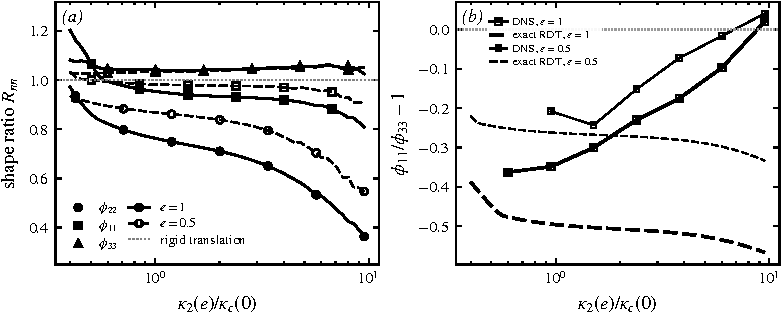
\includegraphics[width=\textwidth]{Figures/fig_rdt_projection.pdf}
  \caption{Exact linear theory does not translate the projected spectra
  rigidly. Left: shape ratio $R_{nn}(\kappa_2)$ of the exactly distorted,
  line-projected component spectra to a rigid translation, at $e=1$ under
  plane strain (closed-form Cauchy solution, isotropic initial fields, four
  realisations). Right: the transverse splitting
  $\phi_{11}/\phi_{33}-1$ versus wavenumber in exact linear theory and in
  the strained-box DNS of \S\,\ref{sec:box-dns}.}
  \label{fig:rdt-projection}
\end{figure}

Two consequences run through the remainder of the paper. First, the
comparison of the full model against the rigid translation
(\S\,\ref{sec:spec-bvc}) measures the departure of the model from its own
kinematics; the departure of the \emph{flow} from linear theory must be
measured against the exact projected reference, and the two differ already
at the linear level. Second, the model's rigid spectral kinematics is
itself a structural approximation---linear theory deepens the projected
anisotropy with wavenumber, which a wavenumber-uniform operator cannot
represent---and \S\,\ref{sec:threeway} quantifies the resulting deficiency
against both the exact reference and DNS.

\begin{figure}
  \centering
  \begin{subfigure}[t]{0.48\textwidth}\centering
    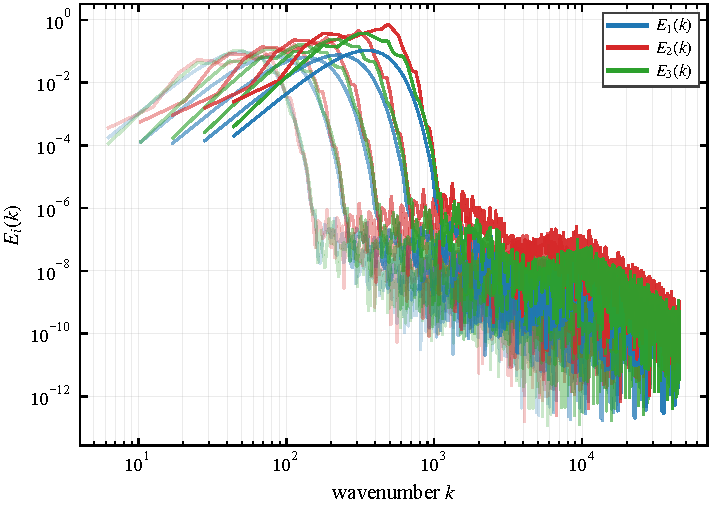
\includegraphics[width=\linewidth]{Figures/fig_spectrum_hs__spectra.pdf}
    \caption{}\label{fig:rdt-spectra}
  \end{subfigure}\hfill
  \begin{subfigure}[t]{0.48\textwidth}\centering
    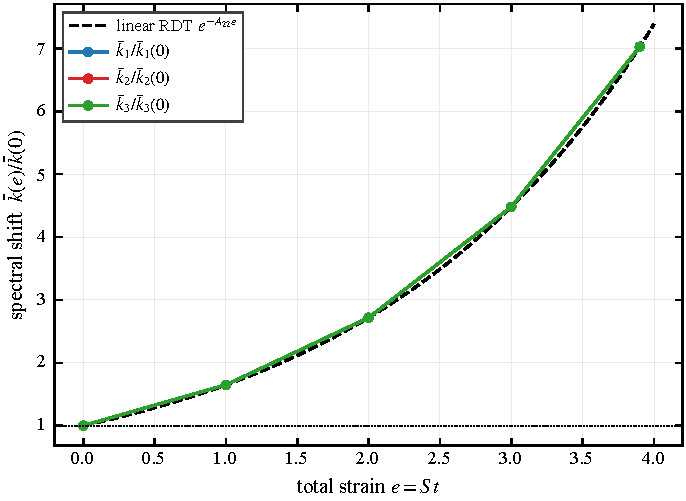
\includegraphics[width=\linewidth]{Figures/fig_spectrum_hs__centroid.pdf}
    \caption{}\label{fig:rdt-centroid}
  \end{subfigure}
  \caption{Compression without cascade (eddy events suppressed, inviscid).
  (\textit{a}) Component spectra $E_i(k)$ at increasing total strain (lighter to
  darker); the spectra translate to higher $k$ without changing shape.
  (\textit{b}) Spectral-centroid migration $\bar k(e)/\bar k(0)$ for each
  component (symbols) against the kinematic prediction $e^{-A_{22}e}$ (dashed).
  The centroid follows the prediction exactly and the three components coincide,
  confirming purely geometric compression of the line.}
  \label{fig:spec-rdt}
\end{figure}

%% TRANSPLANT: V2 sec:spec-bvc (the REFRAMED version, post-M2) — verbatim.
%% TRANSPLANT: V2 sec:cmk (rapid-distortion limit + emergent anisotropy)
%%   — compressed to ~1.5 pp; drop sec:spec-Re and sec:spec-op details to
%%   an appendix table (operating point derivation referenced, not
%%   re-derived).

\emph{[M-spectrum: transplant sec:spec-bvc + compressed CMK here.]}

\subsection{Validation against a strained-box DNS with an exact-RDT
companion}\label{sec:box-dns}

The comparisons above validate the model at the Reynolds-stress level. The
referent quantity for the leading-edge application, however, is spectral,
and the objection that the emergent-spectrum results of
\S\,\ref{sec:val-spectrum} compare the model only with itself must be met
with an independent spectral benchmark under the same strain. To that end
we performed direct numerical simulations of plane-strained homogeneous
turbulence in a deforming-frame (Rogallo-type) pseudo-spectral formulation:
a $128^3$ box, decaying isotropic precursor, then plane strain
$A=S\,\mathrm{diag}(\tfrac12,-\tfrac12,0)$ applied at strain-rate
parameters $Sk_t/\varepsilon\in\{0.8,16\}$ at onset, carried to total
strain $e=1$, four independent realisations
($\kappa_{\max}\eta\approx0.76$ at $e=1$: a pilot resolution, so
small-scale statements below are qualitative). Alongside every DNS
realisation runs an \emph{exact-RDT companion}: the same initial field
evolved under the closed-form Cauchy solution of the linearised equations
and projected onto lines identically to the DNS and to ODT. The companion
is what \S\,\ref{sec:spec-linref} used to construct the linear reference;
here it completes a three-way comparison in which model, linear theory and
DNS are reduced to the same one-dimensional observables. On the ODT side
the ensembles use an unstrained precursor: the line is evolved as ordinary
ODT until the initialisation transient has relaxed and the eddy population
is statistically active, and the strain is switched on only then, so that
the strained evolution starts from a physically conditioned state rather
than from the synthetic initial condition. All ODT statistics in this
subsection are medians over $1024$ realisations per case with bootstrap
confidence intervals; median statistics are used because the strained band
energies are strongly intermittent across realisations, and ensemble means
of spectral ratios are dominated by rare events at any practical sample
size.

\subsubsection{Three-way spectral anisotropy: ODT, exact RDT,
DNS}\label{sec:threeway}

The comparison quantity is the strain-induced change of the spectral
component anisotropy,
$\Delta b_{nn}(\kappa_2)=\phi_{nn}/\sum_m\phi_{mm}-\tfrac13$ at strain $e$,
minus the same quantity evaluated in the system's own unstrained state with
each mode mapped to its strained wavenumber. Referencing each system to its
own $e=0$ state cancels viscous decay, which is component-blind, and the
longitudinal--transverse structure of the isotropic line spectra, which
differs between a three-dimensional box and the component-symmetric ODT
line. Figure~\ref{fig:threeway} and table~\ref{tab:threeway} give the
result at $e=1$, $Sk_t/\varepsilon=0.8$, on common bands of
$\kappa_2(e)/\kappa_c(0)$ with $\kappa_c$ the initial spectral centroid.

\begin{table}
  \centering\small
  \begin{tabular}{lccccccc}
  $\Delta b_{22}(\kappa_2)$, band $\kappa_2/\kappa_c$: & 0.5--0.75 & 0.75--1.2 & 1.2--1.9 & 1.9--3 & 3--4.8 & 4.8--7.6 & 7.6--12\\[2pt]
  exact projected RDT & $+0.146$ & $+0.008$ & $-0.020$ & $-0.041$ & $-0.050$ & $-0.054$ & $-0.056$\\
  DNS                 & $+0.032$ & $-0.033$ & $-0.029$ & $-0.032$ & $-0.036$ & $-0.040$ & $-0.046$\\
  strain-coupled ODT  & $+0.100$ & $+0.101$ & $+0.114$ & $+0.111$ & $+0.127$ & $+0.099$ & $+0.147$\\
  \end{tabular}
  \caption{Strain-induced upwash anisotropy per wavenumber band at $e=1$,
  $Sk_t/\varepsilon=0.8$, each system referenced to its own unstrained
  state. Bands below $0.75\,\kappa_c$ rest on a few box modes and are
  indicative only.}
  \label{tab:threeway}
\end{table}

The structure of the table is the finding. Exact linear theory concentrates
the strain-induced upwash anisotropy at the energy-containing scales and
\emph{removes} it from the small scales, because modes aligned with the
line are amplified least; the DNS shows the same shape, weakened at the
large scales by the nonlinear return. The strain-coupled ODT distributes
its moment-level anisotropy essentially uniformly over wavenumber---the
signature, anticipated in \S\,\ref{sec:spec-linref}, of a
wavenumber-uniform redistribution operator acting on a uniformly dilated
line. The integrated anisotropy is nevertheless correct (the model tracks
the closure at the moment level, \S\,\ref{sec:lr-plane}), so the deficiency
is one of allocation across scales, not of amount. For the leading-edge
application the operative consequence is that the high-wavenumber
anisotropy of the upwash spectrum, which the Amiet response weights, has
the wrong sign in the present model; the closure element that must carry
the correction---a wavenumber-dependent rapid operator in place of the
uniform one---is exactly the spectral kernel formulation of
\S\,\ref{sec:gate}, whose exercise is thereby motivated by a measured
deficit rather than by completeness.

\begin{figure}
  \centering
  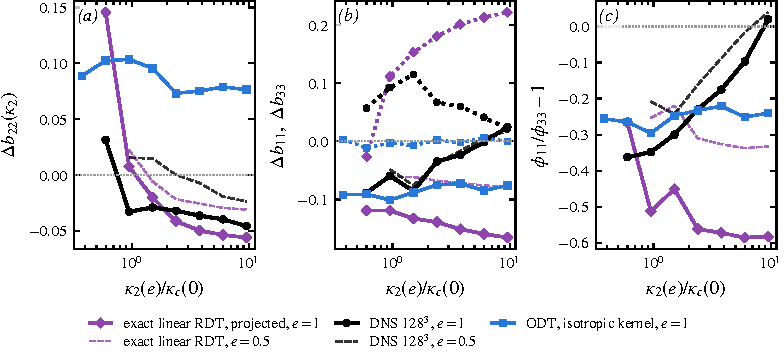
\includegraphics[width=\textwidth]{Figures/fig_threeway.pdf}
  \caption{Three-way comparison at $Sk_t/\varepsilon=0.8$: strain-induced
  anisotropy of the line spectra relative to each system's own unstrained
  state; strain-coupled ODT ($1024$ realisations) against exact projected
  RDT and DNS ($128^3$, four realisations); $e=1$ solid, $e=0.5$ dashed.}
  \label{fig:threeway}
\end{figure}

\subsubsection{Distance from linear theory as a function of strain
rapidity}\label{sec:envelope}

The three-way comparison resolves the anisotropy by wavenumber at one
strain-rate parameter. A complementary scalar measure tracks the
\emph{whole} spectral shape across strain and strain rapidity: at each
total strain the median ODT component line spectra are fitted, jointly in
the upwash and transverse components, by the exactly distorted spectrum of
linear theory---the closed-form Cauchy distortion of an isotropic von
K\'arm\'an field, projected onto the line, with only the pre-distortion
amplitude and energy wavenumber free. The root-mean-square log-residual of
that two-parameter fit is a scale-resolved distance between the model's
strained spectra and exact linear theory. Figure~\ref{fig:rdt-distance}
shows it for precursor-conditioned ensembles at $Sk_t/\varepsilon\approx0.4$
and $\approx8$ at onset ($1024$ realisations each, identical precursor
state: the two fits coincide at $e=0$ at thirteen per cent, the residual
shape mismatch of a relaxed ODT line against the von K\'arm\'an form).

The distance grows with strain in both cases, but \emph{faster at rapid
strain}: to approximately $22$ per cent at $e=2$ for
$Sk_t/\varepsilon\approx0.4$ against approximately $24$ per cent,
saturating early, at $Sk_t/\varepsilon\approx8$, with the separation
established already by $e=0.5$. If the model's rapid response were
spectrally faithful, the rapid curve is the one that should approach zero:
eddy events are subdominant there by construction. That the deviation is
largest precisely where the eddies matter least localises the deficiency in
the rapid kinematics themselves---the wavenumber-uniform operator and the
rigid dilatation---and not in the eddy or relaxation statistics, in
quantitative agreement with the three-way comparison. This measured
validity envelope accompanies the model into any application: predictions
inherit a spectral-shape uncertainty of order the plotted distance at the
operating point's strain and rapidity.

\begin{figure}
  \centering
  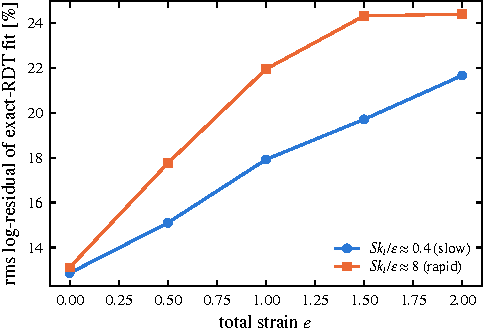
\includegraphics[width=0.62\textwidth]{Figures/fig_rdt_distance.pdf}
  \caption{Scale-resolved distance between the strained ODT line spectra
  and exact linear theory: rms log-residual of the two-parameter
  exact-RDT-distorted von K\'arm\'an fit, against total strain, for slow
  and rapid onset strain-rate parameters (medians over $1024$
  realisations; identical precursor state at $e=0$).}
  \label{fig:rdt-distance}
\end{figure}

% =========================================================================
\section{Closure of the rapid pressure--strain term on a single line}\label{sec:gate}
% =========================================================================
%% THE SPINE.  Rebuild to the six claims of notes/section5_results_note:
%%   1. exact term (Poisson factor 2 — verify V2 eq. 5.3 carries it) +
%%      the obstruction stated exactly        [V2 sec:exact-pi,
%%      sec:obstruction survive ~80%]
%%   2. A1 collapse; A1 exact for axisymmetric distortion, MEASURED under
%%      plane strain (m=2 residue table)      [NEW text from note sec 3-4]
%%   3. LOS estimator: sharp bounds from line data; indeterminacy table;
%%      falsifiers T1/T2                      [NEW from los_estimator note;
%%      forward map + kernels -> Appendix A]
%%   4. reduction to the moment closure; discards kappa-dependence +
%%      ordering                              [V2 sec:lrr-reduction ~70% +
%%      note sec:order for Referee 1.3]
%%   5. rapid/slow disjointness: A=0 null + rapid-limit allocation test
%%                                            [V2 sec:doublecount + note
%%      sec:alloc, compressed]
%%   6. b22(e) linear to e=1, geometry-robust [note sec:dns "control"]
%% Define A1 formally at first use (R3.3).

\emph{[M3: the Section-5 rebuild — the largest single writing task.]}

% =========================================================================
\section{Measured limits, and scale-local relaxation}\label{sec:limits}
% =========================================================================
%% NEW SECTION (the compressed Kerstein arc + envelope interpretation):
%%   - the distance-from-linear-theory envelope (already shown in
%%     sec:envelope) interpreted as the model's validity statement;
%%   - the transmission diagnostic in ONE figure + ONE interventions table
%%     (Options A/A-S/B null; hierarchical kernels levels 1-3: the first
%%     significant fine-scale isotropization, effective where the
%%     sub-scales reach the imbalance, fading under sustained resupply)
%%     [sources: LEN_Extension results_test3: fig_klevels, klevels_table,
%%      facSweep_table, optionA_robust_table; plan doc 4a-4e];
%%   - endpoint: scale-local relaxation is the measured missing
%%     ingredient; the kappa-dependent kernel of sec:gate is the
%%     formulation-level home (exercising eq. 5.7 = map task C3).
%% KEEP TO ~2.5 pp: one figure, one table, no null-result chronicle.

\emph{[M-limits: compressed Kerstein arc — write after Alan's next reply
settles the iterate-vs-depth question, or with current results if the
manuscript moves first.]}

% =========================================================================
\section{Consequence for leading-edge noise}\label{sec:le}
% =========================================================================
%% DETACHABLE (Option C only; write LAST; if length or coherence fails,
%%   this section moves to paper 2 and the introduction's claim shrinks
%%   accordingly).  Sources: LEN_Extension post/acoustics — RDT-vK family
%%   fits (fit_rdt_family), exact Phi_ww(Kx,Ky) from rdt_kernel, Amiet
%%   Delta-SPL chain (gateB_delta_spl); frozen-strain scoping stated
%%   explicitly (R1.4 second half deferred honestly).

\emph{[M5: detachable LE section — decision D1.]}

% =========================================================================
\section{Conclusions}\label{sec:conclusions}
% =========================================================================
%% REWRITE LAST (with abstract).  Must not claim rigid translation as the
%%   linear prediction (old V2 conclusions do).  Claims = abstract's list.

\emph{[M4: conclusions rewrite.]}

% =========================================================================
\appendix
\section{The forward map and the bound kernels}\label{app:forward}
%% TRANSPLANT: los_estimator note sec 2 (derivation of (5.8)-(5.10) —
%%   Referee 3.3's "underived" fixed by deriving them here).
\emph{[Appendix A: transplant from notes/los\_estimator\_note.tex.]}

\section{Numerical parameters and initialisation}\label{app:numerics}
%% TRANSPLANT: V2 implementation details judged supplementary (R1 minor);
%%   the symmetric C^{-1/2} IC whitening statement (correction e);
%%   realization counts and jackknife policy (correction f).
\emph{[Appendix B: numerics + IC whitening + statistics policy.]}

\bibliographystyle{jfm}
\bibliography{jfm}

\end{document}
